\documentclass{beamer}
\mode<presentation>
{
  \usetheme{Warsaw}      % or try Darmstadt, Madrid, Warsaw, ...
  \usecolortheme{beaver} % or try albatross, beaver, crane, ...
  \usefonttheme{default}  % or try serif, structurebold, ...
  \setbeamertemplate{navigation symbols}{}
  \setbeamertemplate{caption}[numbered]
  \setbeamertemplate{footline}[frame number]
}


\usepackage[english]{babel}
\usepackage[utf8]{inputenc}
\usepackage{pgfpages}
\usepackage{algorithm}
\usepackage[noend]{algorithmic}

\title {Real-Time Systems}
\subtitle {The Space of Feasible Execution Times for Asynchronous Periodic Task
Systems using Definitive Idle Times}
\author{Thomas~Chapeaux~\inst{1}~\inst{2} \and Paul~Rodriguez~\inst{1}~\inst{2} \and Laurent~George~\inst{2} \and Joël~Goossens~\inst{1}}
\institute[shortinst]{\inst{1} Université Libre de Bruxelles \and %
                      \inst{2} ECE Paris}
\date{July 2013}

\newcommand{\dbf}[1]{\operatorname{dbf}(#1)}

\begin{document}

\maketitle{}

\begin{frame}
    \tableofcontents[hideothersubsections]
\end{frame}

\section{Introduction}

\begin{frame}
    \tableofcontents[currentsection, hideothersubsections]
\end{frame}

	\subsection{Real-time systems}

	\begin{frame}{Model}
  \begin{block}{Real-Time Systems}
  Systems with real-time constraints. (e.g. ABS, VOD, etc)
  \end{block}
  \textbf{Model:} $\tau$ set of $n$ tasks $\tau_i = (O_i, C_i, D_i, T_i)$ generating jobs $J_{i,j}$
      \begin{itemize}
      \item $O_i$ : arrival of the first job
      \item $C_i$ : execution time
      \item $D_i$ : relative deadline
      \item $T_i$ : time between two job arrivals
    \end{itemize}

  \begin{columns}[c] % the "c" option specifies center vertical alignment
  \column{.4\textwidth}
\begin{center}
\begin{tabular}{|r|c|c|c|c|}
 \hline
  & $O_i$ & $C_i$ & $D_i$ & $T_i$ \\
 \hline
 $\tau_1$ & 1 & 2 & 6 & 10\\
 \hline
 $\tau_2$ & 0 & 3 & 5 & 5\\
 \hline
\end{tabular}
\end{center}

  \column{.6\textwidth} % column designated by a command
\begin{figure}[h]
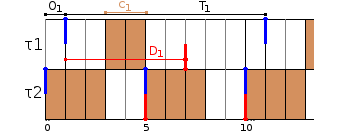
\includegraphics[width=\textwidth]{figs/RTsystem_example.png}
\caption{A task system}
\label{fig:llf}
\end{figure}
  \end{columns}
\end{frame}

    \subsection{Feasibility}

	\begin{frame}{Feasibility}
		\begin{block}{Feasibility}
        A task set is said to be \textbf{feasible} if there exists a schedule such that every job in the task set completes before its deadline is reached.
        \end{block}

        \begin{block}{Feasibility by a scheduling policy}
        A task set is said to be \textbf{schedulable by a given scheduling policy} if every job in the task set completes before its deadline is reached when using this scheduling policy.
        \end{block}

        In the uniprocessor case, the EDF (Earliest Deadline First) scheduling policy is optimal, any feasible task set is EDF-schedulable.
	\end{frame}

    \subsection{C-space}

    \begin{frame}{Definition of the C-space}
        \begin{block}{C-space}
            The \textbf{C-space} of a task system $\tau$ is a region of $n$ dimensions (where each dimension denotes the possible $C_i$ of a task of $\tau$) such that for any vector $C = \{ C_1, \cdots, C_{n}\}$ in it, $\tau$ is feasible.
        \end{block}

        \begin{itemize}
            \item A region of $\mathbb{N}_0^n$ such as the C-space is described by a set of parametric linear constraints
            \item An efficient description allows us to quickly  whether a system whose $O_i$, $T_i$ and $D_i$ values are known will be feasible on a given platform (which gives the $C_i$).
        \end{itemize}

    \end{frame}

	\section{Related works}

    \begin{frame}
    \tableofcontents[currentsection, hideothersubsections]
    \end{frame}

    \subsection{Demand-bound function}

    \begin{frame}{Demand-bound function feasibility test}
        \begin{block}{Demand-bound function}
            The \textbf{demand-bound function (DBF)}
            defined for a task set $\tau$ in a time interval $[t_1, t_2]$, denoted $\dbf{t_1, t_2}$, is
            the maximal cumulated execution time of jobs of $\tau$ contained in the
            closed interval $[t_1, t_2]$.
        \end{block}
        $$\dbf{t_1, t_2} = \sum_{i=1}^{n} n_i(t_1, t_2) \, C_i$$
        where $n_i(t_1, t_2)$ is the number of jobs of task $\tau_i$ whose arrival times
        and deadlines are both in the closed interval $[t_1, t_2]$.

        ~\\

        The following has been shown to be a necessary and sufficient condition of feasibility (called DBF test in the following): $$\dbf{t_1, t_2} \leqslant t_2 - t_1 \; \forall t_1 \leq t_2$$

    \end{frame}

    \subsection{C-space of synchronous systems}

    \begin{frame}{Description using the DBF test}
    The DBF test gives us a set of constraints
    $$\dbf{t_1, t_2} \leqslant t_2 - t_1 \; \forall t_1 \leq t_2$$

    \begin{itemize}
        \item Every constraint is linear in the $C_i$ values
        \item Every constraint is necessary
        \item Their conjunction is sufficient
        % \pause
        \item But we have an infinite number of constraints!
        \item $\Rightarrow$ Removing redundancy
    \end{itemize}
    \end{frame}

    \begin{frame}{Removing redundancy for synchronous system}

    The authors of \cite{george2009characterization} obtain an efficient description of the C-space by
    \begin{itemize}
        \item Removing constraints in which $t_1 > 0$
        \item Removing constraints in which $t_2$ is not a deadline or $t_2 > H$ (where $H = LCM(T_i)$)
    \end{itemize}

    ~\\
    % \pause

    They also define the notion of \textbf{definitive idle times (DIT)} and show that the first one happens at a time $0 < t_d \leqslant H$. Finally they show that all constraints where $t_2 > t_d$ are also redundant.

    ~\\
    % \pause

    The remaining constraints are thus the DBF test on intervals $[0, t]$, where $t$ is a deadline and $0 < t \leqslant t_d$. The remaining redundancies are removed by an algorithm based on the simplex.

    \end{frame}

    % \subsection{Cyclic Idle Times}

    % \begin{frame}{Cyclic Idle Times}

    % \end{frame}

	\subsection{Our work}

	\begin{frame}{Our work}

	In the article, we
    \begin{itemize}
        \item Introduce the notion of \textbf{first periodic DIT (FPDIT)} as a generalization of the notion of DIT
        \item Provide an algorithm to find an efficient description of the C-space for any periodic system
        \item Quantify the feasibility gain of random offsets in terms of C-space volume ratio.
    \end{itemize}

	\end{frame}

\section{First Periodic DIT}

    \begin{frame}
        \tableofcontents[currentsection, hideothersubsections]
    \end{frame}

	\subsection{Definition}

	\begin{frame}{Definition of the FPDIT}
        \begin{block}{Definitive Idle Time}
            A \textbf{definitive idle time} (DIT) \cite{lipariaverage} is a time $t$ (if it exists) such that every job released strictly before instant $t$ has its absolute deadline before or at instant $t$.
        \end{block}

        \begin{block}{First Periodic DIT}
			The \textbf{first periodic DIT} (FPDIT) of a system is the earliest DIT occurring
			strictly after $O_{max}$.
		\end{block}

        The FPDIT is the smallest $t_d$ such as:
       \[
            \begin{array}{l}
                \forall \tau_i \in \tau, \exists a_i \in [D_i,T_i] \; :\\
                \left\{
                    \begin{array}{l}
                        t_d > O_i \\
                        t_d - O_i \equiv a_i \; (mod \; T_i)
                        \\
                    \end{array}
                \right.
            \end{array}
        \]

	\end{frame}

	\subsection{Finding the FPDIT value}

    \begin{frame}{Finding the FPDIT value - Gauss's Algorithm}
        For given values of $a_i$, if the periods are pairwise coprime, equation~(\ref{eq:FPDIT}) has one solution modulo $H$ given by:

        \begin{algorithm}[H]
            \caption{Gauss's CRP Algorithm}
            \label{alg:algoCRP}
            \begin{algorithmic}[1]
                \REQUIRE $C$ the set of constraint $c$ : $\left( t_d \equiv x(c) \; (\operatorname{mod} \; p(c)) \right)$
                \REQUIRE $H$ the hyperperiod of the system
                \FORALL{$c \in C$}
                    \STATE $Mc \leftarrow \frac{H}{p(c)}$
                    \STATE $invMc \leftarrow Mc^{-1} \; (mod \; p(c))$
                    \STATE $e_c \leftarrow Mc \cdot invMc$
                \ENDFOR
                \RETURN $\sum\limits_{c \in C}{x(c) \cdot e_c} \; (mod \; H)$
            \end{algorithmic}
        \end{algorithm}

    \end{frame}

    \begin{frame}{Non-pairwise co-prime moduli}
        If the periods are non-pairwise co-prime, the system has a FPDIT if and only if the following condition is respected:
        \[
            a_i + O_i \equiv a_j + O_j \; (\operatorname{mod} \; \operatorname{gcd}(T_i,
            T_j)) \; \forall i,j
        \]

        Then each equation $t_d \equiv x \; (\operatorname{mod} \; p)$ with $p = p_1^{b_1} \cdots p_k^{b_k}$ (where each $p_i$ is prime), can be replaced by the system:

       \[
            \begin{array}{l}
                \left\{
                    \begin{array}{l}
                         t_d \equiv x \; (mod \; p_1^{b_1}) \\
                         \cdots \\
                         t_d \equiv x \; (mod \; p_k^{b_k})
                    \end{array}
                \right.
            \end{array}
        \]

        Equations with the same $p_i$ can be replaced by only the one of highest $b_i$. The new system now has pairwise co-prime moduli.

    \end{frame}

    \subsection{Frequency of existence}

    \begin{frame}{Frequency of existence of the FPDIT}

    \begin{columns}[c]
        \column{0.4\textwidth}

        Systems were generated by
        \begin{itemize}
            \item Choosing $T_i$ in [5, 20]
            \item Choosing $O_i$ in [0, $H$]
            \item Choosing $D_i$ in [$T_i - CDF * T_i$, $T_i$]
        \end{itemize}

        \column{0.6\textwidth}
        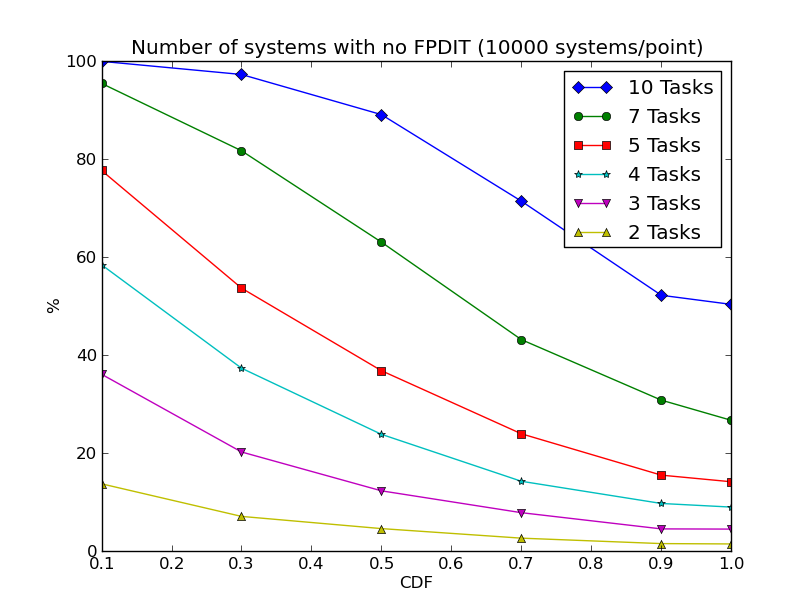
\includegraphics[width=1.2\textwidth]{figs/nofpdit_5.png}

    \end{columns}

    \end{frame}

\section{C-space of asynchronous system}

    \begin{frame}
    \tableofcontents[currentsection, hideothersubsections]
    \end{frame}

    \subsection{Initial description}

	\begin{frame}{Initial description}
		The C-space is still accurately described by the following infinite number of constraints:

        $$\dbf{t_1, t_2} \leq t_2 - t_1 \; \forall t_1 \leqslant  t_2$$

        As in the synchronous case,
        \begin{itemize}
            \item Every constraint is necessary
            \item Their conjunction is sufficient
            \item Most of them are redundant.
        \end{itemize}
        However the method used to remove redundancies will be different.
	\end{frame}

    \subsection{Removing redundancies}

    \begin{frame}{Redundancy as an ILP (I)}

    We can define the redundancy of a linear constraint $C \cdot X \leqslant d$ with regards to a set of $k$ linear constraints $A \cdot X \leqslant B$ as the following Integer Linear Problem (ILP):

    \begin{columns}[c]
        \column{0.1\textwidth}
        \column{0.3\textwidth}

        \begin{block}{Redundancy ILP}

        \begin{center}
        $z = \max \left( C \cdot X \right)$

        s.t.

        $
        \begin{array}{rcc}
          A \cdot X &\leq & B \\
          C \cdot X &\leq & d + 1
        \end{array}
        $
        \end{center}

        \end{block}

        \column{0.1\textwidth}

        \column{0.5\textwidth}

        \begin{center}with\end{center}
        \[
          \begin{array}{ccc}
            A & : & [n,k] \text{ matrix}\\
            B \; \text{and} \; C & : & [n,1] \text{ matrix}\\
            X & : & [1,n] \text{ matrix}\\
            d & : & \text{integer}
          \end{array}
        \]
    \end{columns}
        \begin{itemize}
            \item If $z = d + 1$, the constraint is redundant
            % \item Can be solved with a branch-and-bound approach
            \item Complexity (one test): exponential in the size of the set
            \item Each constraint of the set must be tested
        \end{itemize}

    \end{frame}

    \begin{frame}{Redundancy as an ILP (II)}

        \begin{algorithm}[H]
            \caption{Removing redundant constraints}
            \label{alg:pruneCspace}
          \begin{algorithmic}[1]
            \STATE $CSPACE$ : set of constraints
            \STATE $S \leftarrow \emptyset$
            \STATE \COMMENT{$1^{st}$ pass: test each $cstr$ against previous ones}
            \FOR{$cstr$ \textbf{in} $CSPACE$}
              \IF {$cstr$ is not redundant w.r.t. $S$}
                \STATE $S.push(cstr)$
              \ENDIF
            \ENDFOR
            \STATE \COMMENT{$2^{nd}$ pass: test remaining $cstr$ against every other}
            \FOR{$cstr$ \textbf{in} $S$}
              \STATE $cstr$ = $S.pop()$
              \IF {$cstr$ is not redundant w.r.t. $S$}
                \STATE $S.push(cstr)$
              \ENDIF
            \ENDFOR
            \RETURN{S}
            \end{algorithmic}
        \end{algorithm}

    \end{frame}

    \begin{frame}{Feasibility study interval}

        The authors of \cite{leung1982complexity} have shown that for asynchronous systems, it sufficient to check the DBF test in intervals $[t_1, t_2]$ where $$O_{max} \leqslant t_1 < t_2 \leqslant O_{max} + 2 \cdot H$$

        Indeed, it can be shown that at instant $O_{max} + 2 \cdot H$ at the latest, the system enters a periodic behavior. If follows that if no deadlines have been missed before it, no future deadline misses can occur.

    \end{frame}

    \begin{frame}{Arrivals and deadlines}

        By definition of the demand-bound function, it is sufficient to check only intervals where $t_1$ is an arrival and $t_2$ is a deadline.

        \begin{block}{Demand-bound function}
            The \textbf{demand-bound function (DBF)}
            defined for a task set $\tau$ in a time interval $[t_1, t_2]$, denoted $\dbf{t_1, t_2}$, is
            the maximal cumulated execution time of jobs of $\tau$ contained in the
            closed interval $[t_1, t_2]$.
        \end{block}

    \end{frame}

    \begin{frame}{Using the FPDIT}

        The authors of \cite{choquet2004minimal} define the notion of \emph{cyclic idle times}, the first of which marks the start of the periodic behavior of the system. They prove that if $t_c$ is a cyclic idle time and there are no deadline miss in the interval $[t_c, t_c + H]$, then the system is feasible.

        ~\\

        However the existence and position of the cyclic idle times depend on the values of the $C_i$ and are therefore not accessible when describing the C-space.

        ~\\

        By definition, if the FPDIT exists it will also be a cyclic idle time. It follows that the interval $[t_d, t_d + H]$ is sufficient.

    \end{frame}

    \subsection{Example}

    \begin{frame}{Example (I)}
        \[
        \begin{array}{|r|c|c|c|c|}
         \hline
          & O_i & C_i & D_i & T_i \\
         \hline
         \tau_1 & 8 & C_1 & 7 & 15\\
         \hline
         \tau_2 & 0 & C_2 & 2 & 5\\
         \hline
        \end{array}
        \]

        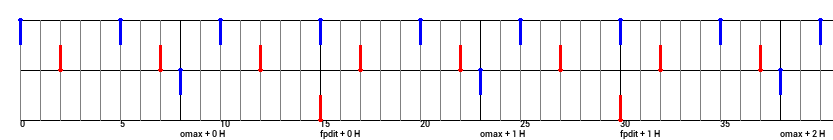
\includegraphics[width=\textwidth]{figs/CspaceExampleArrDead.png}

        \begin{itemize}
            \item $H = 15$
            \item The FPDIT happens at $t_d = 15$
            \item Our study interval is $[15, 30]$ which yields 11 constraints
            \item Without the FPDIT, the interval would be $[8, 38]$ (57 constraints)
        \end{itemize}
    \end{frame}

    \begin{frame}{Example (II)}

    We remove the remaining redundancies with the ILP:
    $$
        \left\{
            \begin{array}{cccccc}
                & & & C_2 & \leqslant & 2 \\
                C_1 & + & & C_2 & \leqslant & 7
            \end{array}
        \right.
    $$

    The C-space of the corresponding synchronous system is:
    $$
    \left\{
      \begin{array}{cccccc}
        & & & C_2 & \leqslant & 2 \\
        C_1 & + & 2 & C_2 & \leqslant & 7
      \end{array}
    \right.
    $$

    \begin{columns}[c]

    \column{0.5\textwidth}

    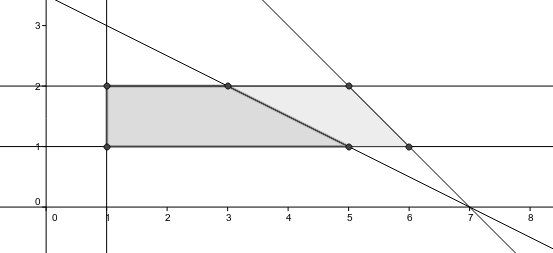
\includegraphics[width=\textwidth]{figs/cspace_example.png}

    \column{0.5\textwidth}

    The offsets allow three more $C_i$ values to be feasible.

    \end{columns}

    \end{frame}

\section{Feasibility gain of random offsets}

    \begin{frame}
    \tableofcontents[currentsection, hideothersubsections]
    \end{frame}

    \begin{frame}{Experiment}

        We want to express the feasibility gain of random offsets as the ratio

        $$\frac{V(\tau)}{V(\tau')}$$

        Where
        \begin{itemize}
            \item $\tau$ is a synchronous system
            \item $\tau'$ is $\tau$ with added offsets
            \item $V(\tau)$ is the size of the C-space of $\tau$
        \end{itemize}

    \end{frame}

    \begin{frame}{Result}

        \begin{columns}[c]

        \column{0.5\textwidth}

            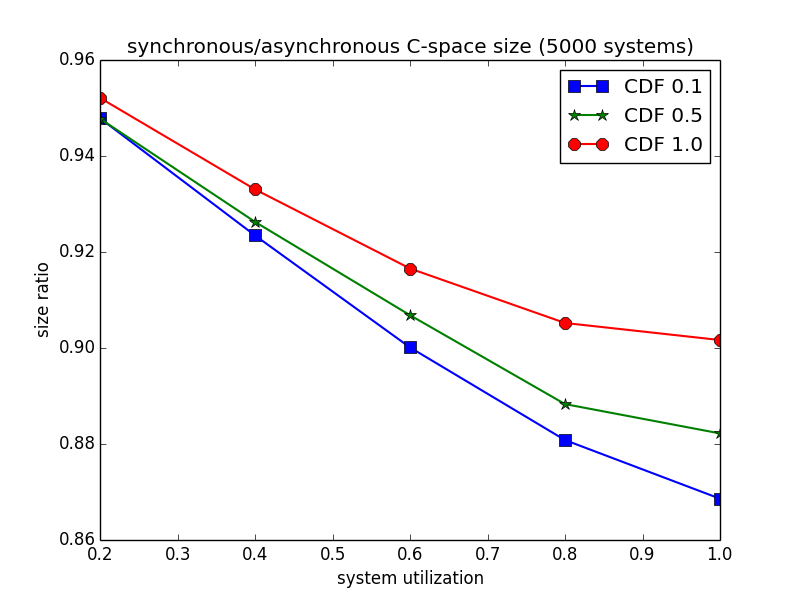
\includegraphics[width=1.2\textwidth]{figs/sizeratio.png}

        \column{0.5\textwidth}

            \begin{itemize}
                \item Around 10\% of amelioration for high-utilization systems
                \item Gain not highly dependent of utilization or CDF
            \end{itemize}

        \end{columns}

    \end{frame}

\section{Future Works}

    \begin{frame}{Future Works}

    \begin{itemize}
        \item Further ways of reducing redundancy before applying the simplex
        \item Other metrics to quantify the quality of the C-space
        \item Extension to multiprocessor scheduling
    \end{itemize}

    \end{frame}

\bibliographystyle{IEEEtran}
\bibliography{dit-paper}

\end{document}

